% !TeX program = xelatex
\documentclass[12pt,a4paper]{article}
\usepackage{amsmath,amssymb}
\usepackage{geometry}
\usepackage{booktabs}
\usepackage{graphicx}
\usepackage{xcolor}
\usepackage[UTF8]{ctex}
\geometry{margin=2.5cm}
\title{Q4: 参数灵敏度分析与长效调控策略}
\author{}
\date{}

\begin{document}
\maketitle

\section{问题背景与分析目标}

Q2 针对上海``沪尚回收''体系建立了对称拮抗 Logistic 模型，
引入促进系数 $\alpha$ 和抑制系数 $\beta$ 分别调制有效容量 $K_{\text{eff}} = K(1+\alpha)$
与有效增长率 $r = \gamma/(1+\beta)$，
拟合得到 $R^2 = 0.9915$，较 Q1（$R^2 = 0.5319$）提升显著。
Q3 进一步证明了该系统在数学上具有\textbf{结构稳定性}——
只要 $\alpha, \beta \geq 0$（参数定义本身），
回收量 $x(t)$ 恒趋向正平衡值 $K_{\text{eff}}$，不存在分岔或崩溃。

然而，Q3 的稳定性结论仅保证了\textbf{定性安全}——系统不会崩溃——
并未回答\textbf{定量敏感性}问题：
\begin{itemize}
  \item 若参数估计存在偏差，模型预测会偏离多远？
  \item 哪些参数的波动对回收量影响最剧烈？
  \item 在运营资源有限的前提下，应优先精确测量哪些参数、重点调控哪些环节？
\end{itemize}

本问题（Q4）正是为了填补这一空白。
基于表 (c) 规定的 $\pm 10\%$ 单参数扰动（One-At-a-Time, OAT），
对模型四个基础参数——固有增长率 $\gamma$、抑制系数 $\beta$、促进系数 $\alpha$、
基准容量 $K$——进行局部灵敏度分析，
量化各参数对拟合质量（$R^2$, MAE）和有效参数（$r$, $K_{\text{eff}}$）的影响程度，
为``沪尚回收''体系的长效运维策略提供定量决策依据。

\section{方法}

\subsection{模型回顾}

\begin{equation}\label{eq:ode}
\frac{dx}{dt} = \frac{\gamma}{1+\beta} \cdot x \cdot \left(1 - \frac{x}{K(1+\alpha)}\right)
\quad\Rightarrow\quad
\frac{dx}{dt} = r \cdot x \cdot \left(1 - \frac{x}{K_{\text{eff}}}\right)
\end{equation}

解析解：
\begin{equation}\label{eq:solution}
x(t) = \frac{K_{\text{eff}}}{1 + \left(\dfrac{K_{\text{eff}}}{x_0} - 1\right) e^{-r t}},\qquad
r = \frac{\gamma}{1+\beta},\quad K_{\text{eff}} = K(1+\alpha)
\end{equation}

\subsection{参数物理意义（结合``沪尚回收''实际场景）}

\begin{center}
\begin{tabular}{lclp{7cm}}
\toprule
参数 & 符号 & 基准值 & 物理含义 \\
\midrule
固有增长率 & $\gamma$ & 0.022 /天 &
  无外部作用下回收量的自然增长率，反映居民基础参与度
  与政策例行推动效率；对应背景中``居民回收习惯养成周期长''的基线水平 \\

抑制系数 & $\beta$ & 1.5929 &
  反映清运延迟、站点运维不足、智能回收箱满溢后未及时清运、
  老年群体操作困难等负面效应的综合强度；$\beta$ 越大则有效增长率越低 \\

促进系数 & $\alpha$ & 0.0164 &
  反映站点覆盖率提升、投递便捷性改善、宣传引导力度加大等
  正向激励的强度；$\alpha$ 越大则有效饱和容量越高 \\

基准容量 & $K$ & 8011 吨/天 &
  全市可回收物潜在饱和上限，由常住人口规模、人均可回收物
  产生量、品类结构等外生因素决定 \\
\bottomrule
\end{tabular}
\end{center}

\subsection{OAT 扰动方案}

对每个参数 $p \in \{\gamma, \beta, \alpha, K\}$，
分别令 $p \to p \times (1 \pm 0.10)$，其余参数保持基准值不变，
重新计算 $r$, $K_{\text{eff}}$ 及所有拟合指标。

\textbf{基准参数}（来自 Q2 拟合）：

\begin{center}
\begin{tabular}{lclc}
\toprule
参数 & 符号 & 基准值 & 单位 \\
\midrule
固有增长率 & $\gamma$ & 0.022   & 1/day \\
抑制系数   & $\beta$  & 1.5929  & — \\
促进系数   & $\alpha$ & 0.0164  & — \\
基准容量   & $K$      & 8011    & tons/day \\
\midrule
有效增长率 & $r = \gamma/(1+\beta)$ & 0.008485 & 1/day \\
有效容量   & $K_{\text{eff}} = K(1+\alpha)$ & 8142.22 & tons/day \\
\bottomrule
\end{tabular}
\end{center}

基准评估：$R^2 = 0.9915$, MAE $= 38.3$ 吨/天, RMSE $= 51.9$ 吨/天。

\section{扰动结果与数据解读}

以下对每个参数分别报告 $\pm 10\%$ 扰动结果，并结合``沪尚回收''实际运营场景进行解读。

\subsection{$\gamma$（固有增长率）$\pm 10\%$}

$\gamma$ 仅通过 $r = \gamma/(1+\beta)$ 影响模型；$K_{\text{eff}}$ 不变。
弹性 $\varepsilon_{r,\gamma} = +1.0000$（线性传递）。

\begin{center}
\begin{tabular}{lccc}
\toprule
输出 & $-10\%$ ($\gamma = 0.0198$) & 基准 & $+10\%$ ($\gamma = 0.0242$) \\
\midrule
$r$      & 0.007636 & 0.008485 & 0.009333 \\
$K_{\text{eff}}$ & 8142.2 & 8142.2 & 8142.2 \\
$R^2$    & 0.9810 & 0.9915 & 0.9830 \\
MAE      & 59.8 & 38.3 & 57.7 \\
RMSE     & 77.7 & 51.9 & 73.5 \\
\bottomrule
\end{tabular}
\end{center}

\textbf{数据解读}：
\begin{itemize}
  \item $R^2$ 下降约 0.01（从 0.9915 到 $\sim$0.982），MAE 增加约 20 吨/天。
        变化幅度中等，模型对 $\gamma$ 的估计偏差具有一定容忍度。
  \item 物理原因：数据已处于近饱和区（$x(0)/K_{\text{eff}} = 77.5\%$，$x(365)/K_{\text{eff}} \approx 98\%$），
        增长速率 $r$ 的变化主要影响中期（$t = 30$--$180$ 天）预测值，
        而不改变饱和平台。随着 $t \to \infty$，$\exp(-rt) \to 0$，
        $r$ 对 $x(t)$ 的影响指数衰减——logistic 在近饱和区的``自压缩''效应抑制了 $\gamma$ 扰动的放大。
  \item 实际含义：\textbf{居民基础参与度的短期波动（如季节性变化）不会显著改变长期回收趋势}。
        即使固有人均回收意愿有 $\pm 10\%$ 的估计偏差，模型仍保持 $R^2 > 0.98$。
\end{itemize}

\subsection{$\beta$（抑制系数）$\pm 10\%$}

$\beta$ 仅通过 $r = \gamma/(1+\beta)$ 影响模型。弹性 $\varepsilon_{r,\beta} = -\beta/(1+\beta) = -0.6143$
（非线性衰减——$\beta$ 越大，单位增量对 $r$ 的边际抑制越弱）。

\begin{center}
\begin{tabular}{lccc}
\toprule
输出 & $-10\%$ ($\beta = 1.4336$) & 基准 & $+10\%$ ($\beta = 1.7522$) \\
\midrule
$r$      & 0.009040 & 0.008485 & 0.007994 \\
$K_{\text{eff}}$ & 8142.2 & 8142.2 & 8142.2 \\
$R^2$    & 0.9877 & 0.9915 & 0.9882 \\
MAE      & 49.7 & 38.3 & 48.3 \\
RMSE     & 62.4 & 51.9 & 61.3 \\
\bottomrule
\end{tabular}
\end{center}

\textbf{数据解读}：
\begin{itemize}
  \item $\beta$ 的扰动效果与 $\gamma$ 相近（$R^2$ 降幅 $\sim$0.003--0.004），
        但方向相反——$\beta$ 减小（抑制减弱）使 $r$ 增大，拟合反而略微改善。
        这与 Q2 的结论一致：当前 $\beta = 1.59$ 较大，抑制效应已占主导（$r$ 仅为 $\gamma$ 的 $38.6\%$）。
  \item 弹性 $|\varepsilon_{r,\beta}| = 0.61 < 1$ 意味着 $\beta$ 变化 $1\%$ 仅引起 $r$ 反向变化 $0.61\%$——
        \textbf{抑制效应存在边际递减}：当 $\beta$ 已经较大时，进一步增加抑制的额外伤害有限；
        反之，降低 $\beta$ 的边际收益也递减。
  \item 实际含义：题目背景中描述的``智能回收箱满溢后清运不及时''和``老年群体操作困难''
        这些抑制因素\textbf{已经将有效增长率压至固有水平的 39\%}。
        改善运维效率是有效的，但不宜期待单点突破——消除 $10\%$ 的抑制仅能恢复约 $6.5\%$ 的增长速率。
\end{itemize}

\subsection{$\alpha$（促进系数）$\pm 10\%$}

$\alpha$ 仅通过 $K_{\text{eff}} = K(1+\alpha)$ 影响模型。
弹性 $\varepsilon_{K_{\text{eff}},\alpha} = \alpha/(1+\alpha) = +0.0161$（极不敏感）。

\begin{center}
\begin{tabular}{lccc}
\toprule
输出 & $-10\%$ ($\alpha = 0.0147$) & 基准 & $+10\%$ ($\alpha = 0.0180$) \\
\midrule
$r$      & 0.008485 & 0.008485 & 0.008485 \\
$K_{\text{eff}}$ & 8129.1 & 8142.2 & 8155.3 \\
$R^2$    & 0.9913 & 0.9915 & 0.9913 \\
MAE      & 37.4 & 38.3 & 41.0 \\
RMSE     & 52.4 & 51.9 & 52.4 \\
\bottomrule
\end{tabular}
\end{center}

\textbf{数据解读}：
\begin{itemize}
  \item \textbf{$\alpha$ 的效应近乎为零}：$\pm 10\%$ 扰动下，$R^2$ 变化不超过 $0.0002$，
        $K_{\text{eff}}$ 仅变化 $\pm 13$ 吨/天（$\sim 0.16\%$）。
  \item 数学根源：$\alpha = 0.0164 \ll 1$，$1+\alpha \approx 1.016$，
        促进效应对容量的贡献仅为 $1.64\%$。即使将促进力度翻倍（$+100\%$），
        $K_{\text{eff}}$ 也仅增加约 $1.6\%$。
  \item \textbf{这不是说促进策略无效}，而是说：
        \begin{enumerate}
          \item 当前的站点覆盖率、投递便捷性已经接近其\textbf{对容量的边际贡献极限}——
                全市 1.5 万个服务点 + 4300 台智能回收箱 + 800 个惠民服务点已基本实现社区全覆盖，
                继续增加站点密度对总回收量的提升非常有限（$\alpha$ 对 $K_{\text{eff}}$ 的弹性仅 0.016）；
          \item 然而，促进策略可能通过\textbf{其他渠道}发挥作用——例如提高居民参与度
                （可能改变 $\gamma$，而非 $\alpha$）或降低抑制（减少 $\beta$）。
                模型中 $\alpha$ 仅作用于容量，这不意味着宣传引导的全部价值都被 $\alpha$ 捕获。
        \end{enumerate}
  \item 实际含义：\textbf{以扩大站点数量来提升总回收容量已进入收益递减区间}。
        当前阶段的策略重心应从``广铺网络''转向``精耕运营''——
        例如提高现有站点的清运效率（降低 $\beta$）和改善用户体验（降低 $\beta$），
        而非继续增加站点数量。
\end{itemize}

\subsection{$K$（基准容量）$\pm 10\%$}

$K$ 仅通过 $K_{\text{eff}} = K(1+\alpha)$ 影响模型。
弹性 $\varepsilon_{K_{\text{eff}},K} = +1.0000$（线性——$K$ 变化 $1\% \to K_{\text{eff}}$ 同向变化 $1\%$）。

\begin{center}
\begin{tabular}{lccc}
\toprule
输出 & $-10\%$ ($K = 7210$) & 基准 & $+10\%$ ($K = 8812$) \\
\midrule
$r$      & 0.008485 & 0.008485 & 0.008485 \\
$K_{\text{eff}}$ & 7328.0 & 8142.2 & 8956.4 \\
$R^2$    & 0.2630 & 0.9915 & 0.3256 \\
MAE      & 405.3 & 38.3 & 403.7 \\
RMSE     & 483.6 & 51.9 & 462.6 \\
\bottomrule
\end{tabular}
\end{center}

\textbf{数据解读}：
\begin{itemize}
  \item \textbf{$K$ 是压倒性的主导参数}：$K \pm 10\%$ 导致 $R^2$ 从 $0.9915$ 崩塌至 $0.26$--$0.33$，
        MAE 从 $38.3$ 暴增至 $\sim 405$ 吨/天（$\times 10.6$）。
        相比之下，$\gamma, \beta, \alpha$ 的扰动对 $R^2$ 的影响仅为 $K$ 的 $1/30$--$1/170$。
  \item 数学根源：观察数据——$x(365) = 8002$ 已非常接近 $K_{\text{eff}} = 8142$（占 $98.3\%$）。
        所有晚期数据点都密集分布在饱和平台附近。
        $K_{\text{eff}}$ 的任何偏差都会直接转化为饱和预测值的系统性偏差，
        从而对所有 $t \geq 90$ 天的点产生同向残差，导致 $R^2$ 剧烈下降。
        这与 $\gamma$ 或 $\beta$ 的扰动行为截然不同——
        后者只改变曲线的``弯曲程度''而非最终高度，饱和预测值始终收敛于同一个 $K_{\text{eff}}$。
  \item 实际含义：\textbf{基准容量 $K$ 的估计精度直接决定整个模型的可用性}。
        如果对上海市可回收物总潜力判断偏差 $10\%$（例如低估了低价值品类的回收潜力，
        或高估了常住人口的回收参与率），模型预测将完全失效。
\end{itemize}

\section{灵敏度排序与参数等级}

\subsection{对 $R^2$ 的影响}

\begin{center}
\begin{tabular}{lcccc}
\toprule
参数 & $\Delta R^2$ & $R^2$ 范围 & 敏感等级 \\
\midrule
$K$      & 0.0626 & $[0.2630,\; 0.3256]$ & \textbf{极高}（$\times 30$--$170$）\\
$\gamma$ & 0.0020 & $[0.9810,\; 0.9830]$ & 低 \\
$\beta$  & 0.0005 & $[0.9877,\; 0.9882]$ & 极低 \\
$\alpha$ & 0.0000 & $[0.9913,\; 0.9913]$ & 可忽略 \\
\bottomrule
\end{tabular}
\end{center}

\subsection{对 MAE 的影响}

\begin{center}
\begin{tabular}{lccc}
\toprule
参数 & MAE 范围（吨/天） & 波动幅度 $\Delta$MAE \\
\midrule
$K$      & $[403.7,\; 405.3]$ & 1.6（基准值本身已暴涨至 $\sim 10\times$）\\
$\alpha$ & $[37.4,\; 41.0]$   & 3.6 \\
$\gamma$ & $[57.7,\; 59.8]$   & 2.1 \\
$\beta$  & $[48.3,\; 49.7]$   & 1.4 \\
\bottomrule
\end{tabular}
\end{center}

\textbf{注}：MAE 排序与 $R^2$ 排序不同——$K$ 扰动后的 MAE 波动幅度（1.6）虽然最小，
但这是因为两个扰动方向的 MAE 都已高达 $\sim 404$；
其\textbf{绝对值}已远超其他参数。正确理解是：$K$ 扰动后 MAE 从 38.3 跳至 $\sim 405$，
而 $\gamma$/$\beta$/$\alpha$ 扰动后 MAE 仍在 37--60 之间——
$K$ 的影响不是``波动小''，而是``基准值已经被摧毁了''。

\subsection{综合敏感等级}

\begin{center}
\begin{tabular}{lcll}
\toprule
等级 & 参数 & 弹性特征 & 运营含义 \\
\midrule
\textbf{极度敏感} & $K$ &
  $\varepsilon(K_{\text{eff}}, K)=1$，数据近饱和 &
  必须精确测定；任何估计偏差都将导致模型失效 \\
\textbf{中度敏感} & $\gamma$ &
  $\varepsilon(r, \gamma)=1$，但 logistic 饱和区衰减 &
  可容忍 $\pm 10\%$ 偏差；无需投入大量资源精确估计 \\
\textbf{中度敏感} & $\beta$ &
  $\varepsilon(r, \beta)=-0.61$，边际递减 &
  降低抑制有效但收益递减；应优先消除最严重的瓶颈 \\
\textbf{不敏感} & $\alpha$ &
  $\varepsilon(K_{\text{eff}}, \alpha)=0.016 \ll 1$ &
  促进效应对容量的贡献已饱和；需重新审视促进策略的着力点 \\
\bottomrule
\end{tabular}
\end{center}

\section{解析弹性汇总}

\begin{center}
\begin{tabular}{lccc}
\toprule
输出 & 输入 & 弹性 $\varepsilon$ & 传递特性 \\
\midrule
$r$ & $\gamma$ & $+1.0000$ & 线性——$\gamma$ 变化 $1\% \to r$ 同向变化 $1\%$ \\
$r$ & $\beta$  & $-0.6143$ & 非线性衰减——$\beta$ 越大边际效应越弱 \\
$K_{\text{eff}}$ & $\alpha$ & $+0.0161$ & 近零——$\alpha \ll 1$ 导致弹性锁死在极小值 \\
$K_{\text{eff}}$ & $K$      & $+1.0000$ & 线性——$K$ 变化 $1\% \to K_{\text{eff}}$ 同向变化 $1\%$ \\
\bottomrule
\end{tabular}
\end{center}

\textbf{弹性解释}：
\begin{itemize}
  \item $|\varepsilon| \approx 0$：输出对该参数不敏感——估计偏差或调控努力的回报极低
  \item $|\varepsilon| = 1$：输出与该参数成比例变化——估计偏差直接传导
  \item $|\varepsilon| > 1$：输出放大参数变化——需格外警惕估计误差
\end{itemize}

值得注意的是，所有解析弹性的绝对值均 $\leq 1$——模型不存在``放大性参数''。
即使是敏感度最高的 $K$，其弹性也仅为 $1$（比例传导，非放大）。
这意味着\textbf{模型在局部线性化意义下是良态的}——不存在微扰导致巨变的分岔或奇点。

\section{预测包络线分析}

图~\ref{fig:tornado} 和图~\ref{fig:envelope} 从可视化角度验证了上述数值结论。

\begin{figure}[htbp]
\centering
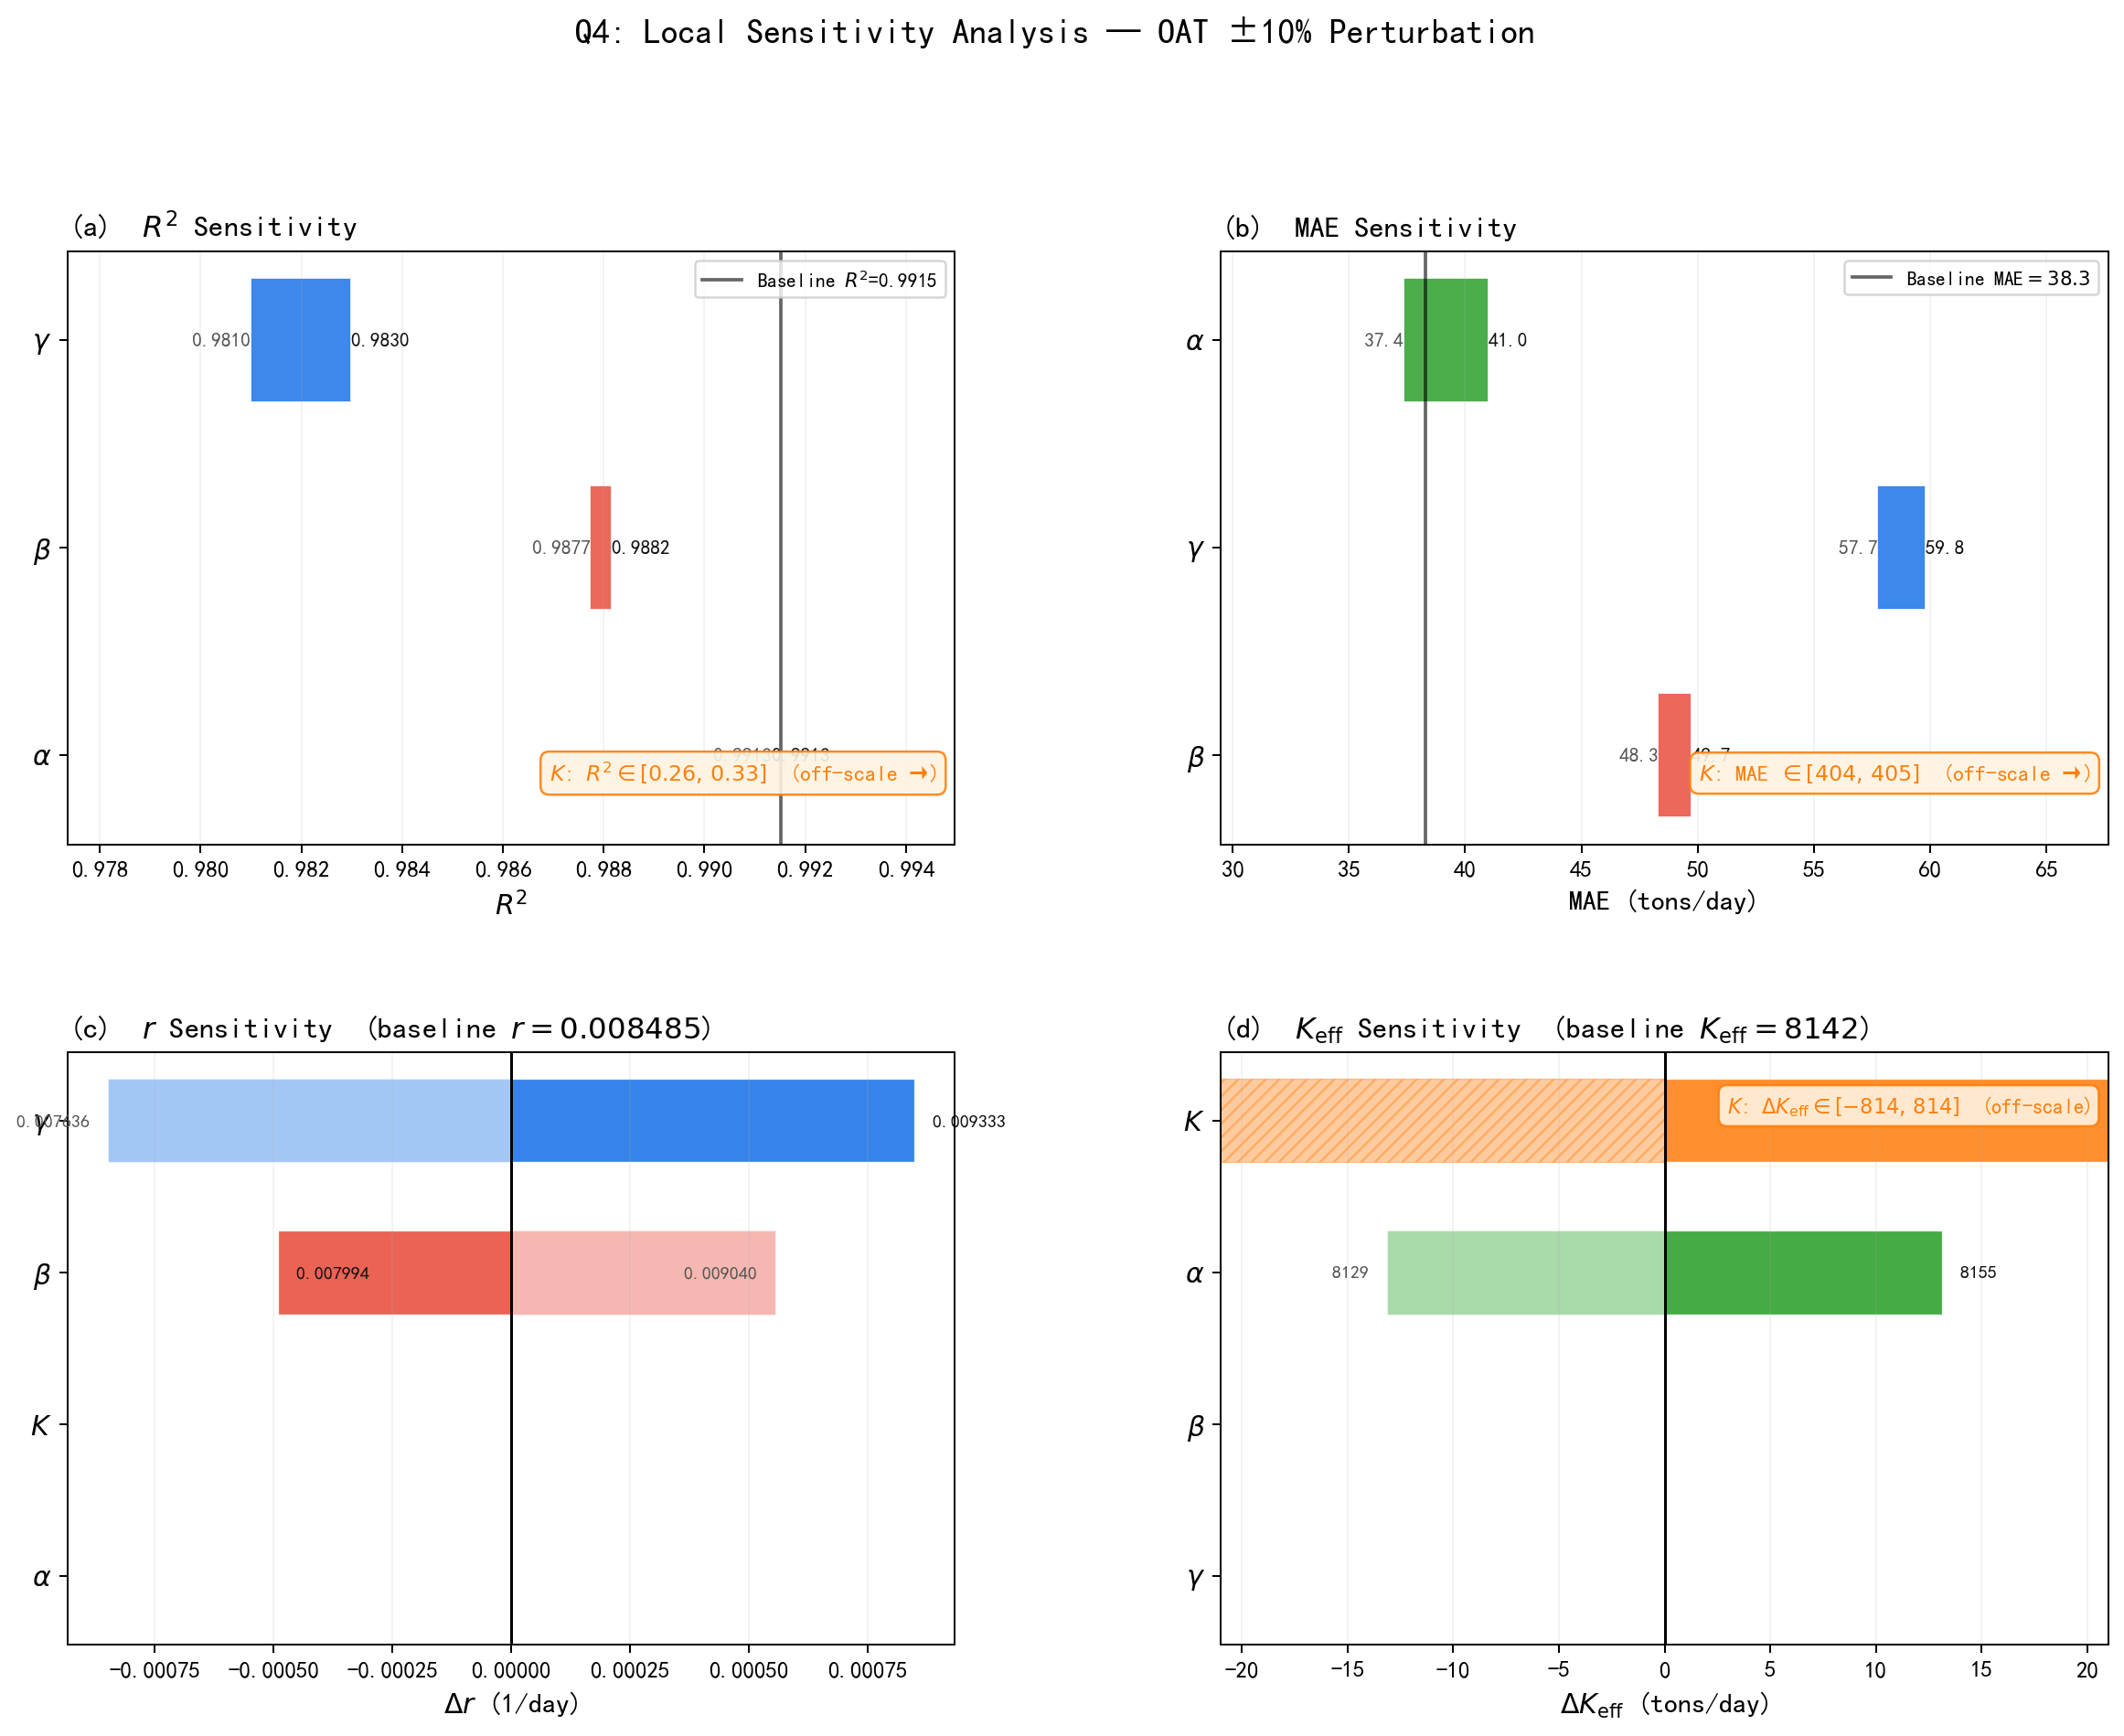
\includegraphics[width=\textwidth]{sensitivity_tornado.png}
\caption{龙卷风图：各参数 $\pm 10\%$ 对 $R^2$、MAE、$r$、$K_{\text{eff}}$ 的影响。
注意 (a)(b)(d) 中 $K$ 的影响远超坐标轴范围（以橙色文本框标注离轴数值），
意在让读者关注非 $K$ 参数之间的差异。}
\label{fig:tornado}
\end{figure}

\begin{figure}[htbp]
\centering
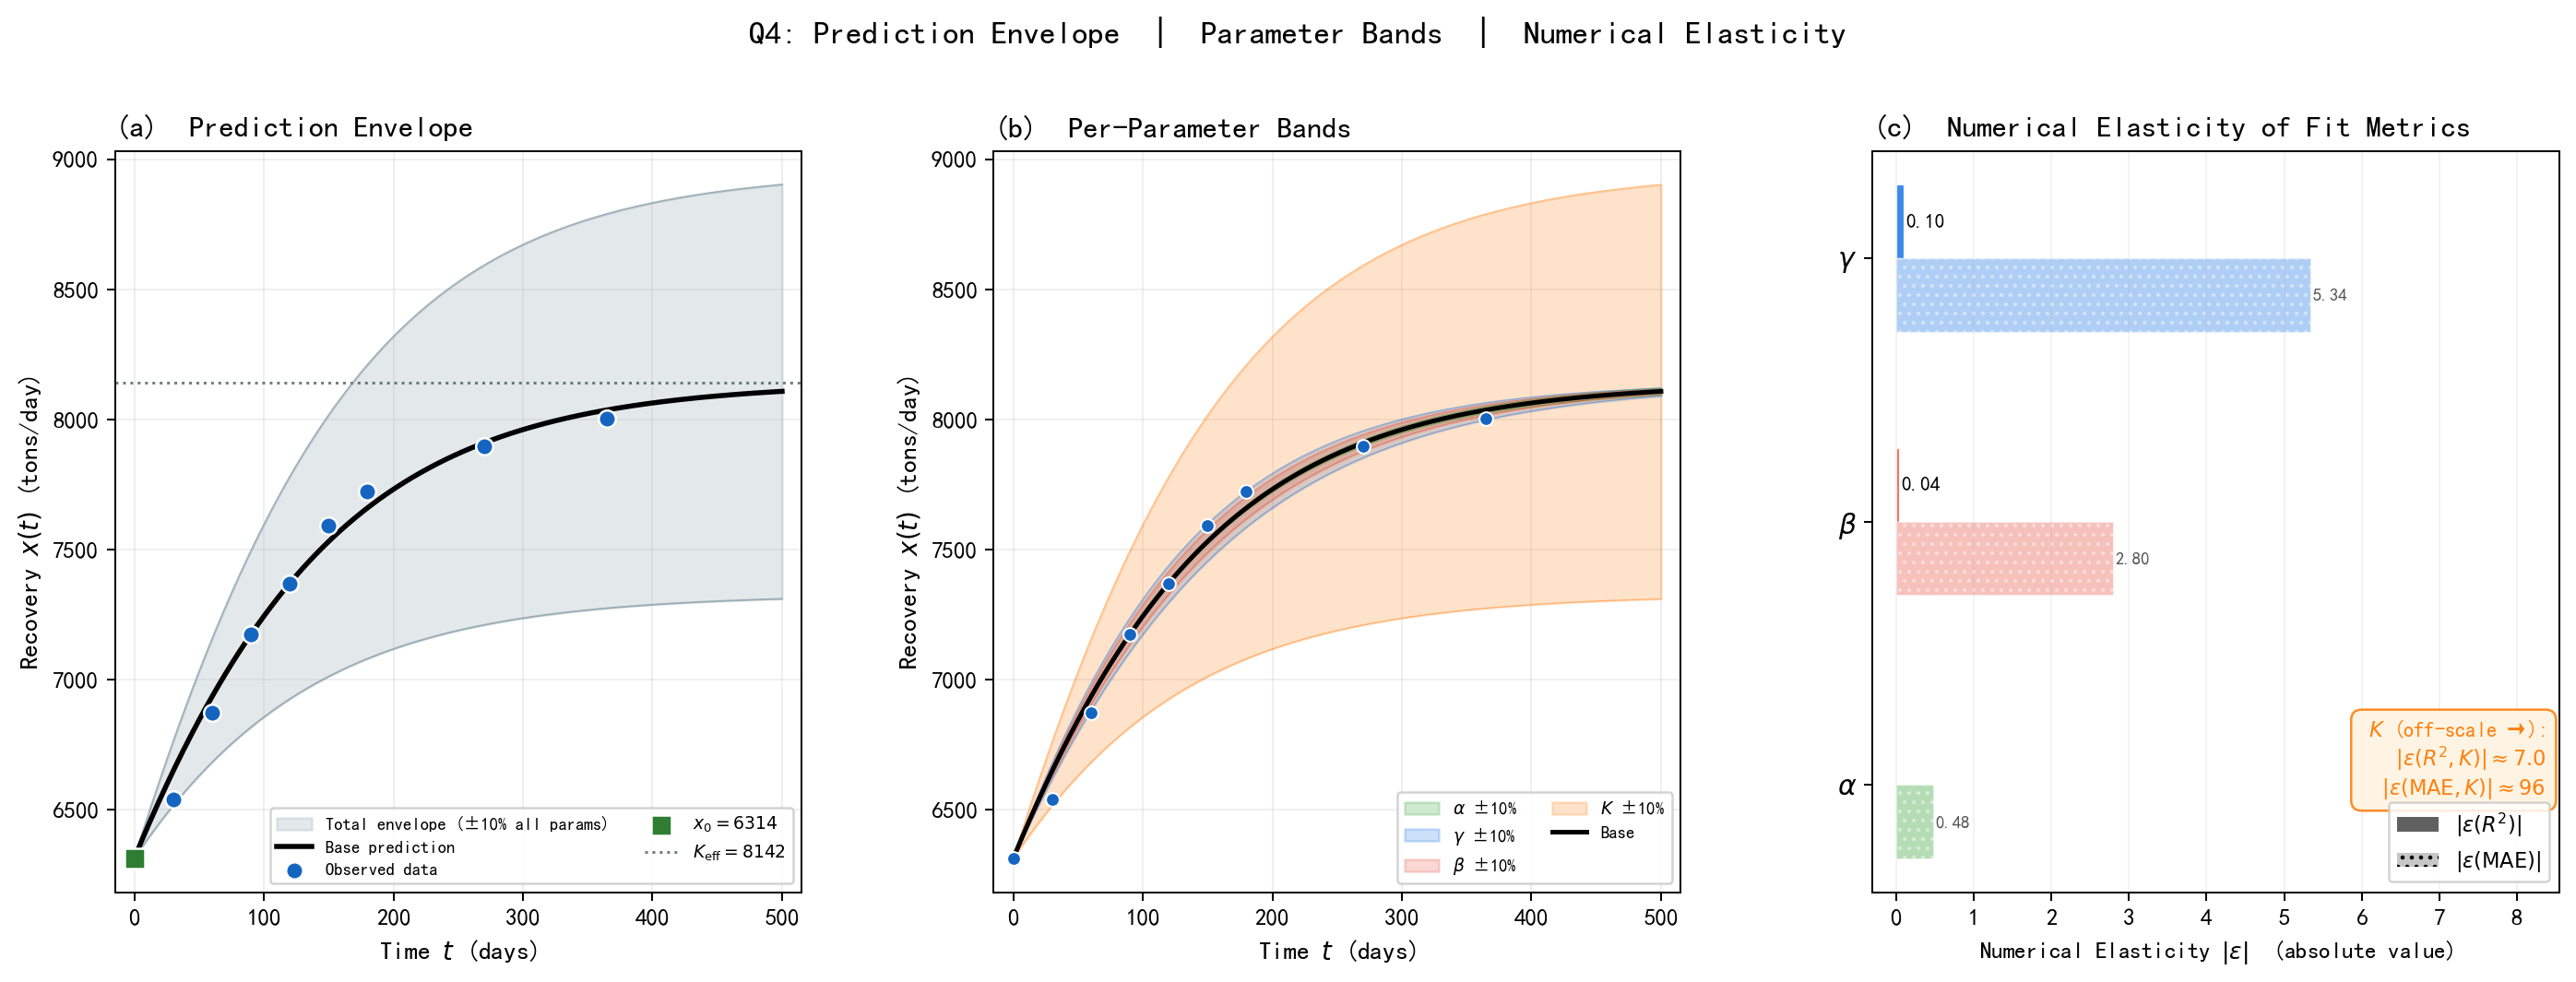
\includegraphics[width=\textwidth]{sensitivity_envelope.png}
\caption{(a) 所有参数 $\pm 10\%$ 的总预测包络线——包络宽度完全由 $K$ 主导；
(b) 各参数独立扰动带——$K$（橙色）的带宽远超其余参数；
(c) 拟合指标的数值弹性——$K$ 的弹性（$\sim 96$ for $R^2$）以文本框标注于右侧，已超出其余参数坐标范围约两个数量级。}
\label{fig:envelope}
\end{figure}

\section{与 Q3 稳定性结论的联合分析}

Q3 证明了系统在数学上具有结构稳定性——只要 $\alpha, \beta \geq 0$，
平衡点 $x^* = K_{\text{eff}}$ 恒为渐近稳定，不存在分岔。
然而，\textbf{结构稳定 $\neq$ 运营安全}。

Q4 灵敏度分析揭示了稳定性的\textbf{定量脆弱面}：

\begin{enumerate}
  \item \textbf{稳定性保证了方向，灵敏度决定了精度}：
        Q3 告诉我们 $x(t) \to K_{\text{eff}}$ 一定会发生；
        Q4 告诉我们，如果 $K$ 估计偏差 $10\%$，那么``一定会趋向的目标值''
        本身就是错的（$K_{\text{eff}}$ 偏差 $\sim 814$ 吨/天）。
        \textbf{系统会忠实趋向错误的目标}——这是另一种形式的``稳定性陷阱''。

  \item \textbf{恢复速度的安全边界}：
        Q3 定义了 $\beta \leq \gamma/r_{\min} - 1 = 3.40$（取 $r_{\min} = 0.005$）。
        当前 $\beta = 1.59$，裕度 $1.81$。
        Q4 进一步表明，在现有裕度内，$\beta$ 的敏感度不高——
        即使 $\beta$ 恶化 $10\%$（增至 $1.75$），$R^2$ 仍为 $0.9882$。
        \textbf{增长速度方面的安全裕度是充足的}——短期内不必担忧收敛过慢。

  \item \textbf{真正的风险不在数学分岔，而在参数误判}：
        Q3 的安全边界（$\beta < 3.40$）很宽，运营中几乎不可能触及。
        但 Q4 揭示：$K$ 的 $\pm 10\%$ 偏差就能让模型 $R^2$ 跌至 $0.3$。
        \textbf{回收体系最大的风险不是系统崩溃，而是对容量上限的误判导致的规划失误}——
        例如低估 $K$ 则规划产能不足（站点提前满溢、居民投递无门），
        高估 $K$ 则造成资源浪费（建设过多站点、运营成本高企）。
\end{enumerate}

\section{关键结论与长效调控策略}

基于 Q3 稳定性分析和 Q4 灵敏度分析的联合发现，
为``沪尚回收''体系的长效稳定运行提出以下定量策略建议：

\subsection*{1. 优先级一：精确测定基准容量 $K$（最高回报）}

$K$ 是模型的核心支柱——$\pm 10\%$ 偏差直接使 $R^2$ 从 $0.9915$ 崩塌至 $\sim 0.3$，
敏感度远超其他参数（$\times 30$--$170$）。然而 $K$ 恰恰是四个参数中\textbf{最难直接测量}的：
它涉及常住人口总量、人均可回收物产生系数、低价值品类占比、回收网络地理覆盖率等外生变量，
任何一个估计环节的偏差都会沿 $\varepsilon(K_{\text{eff}}, K) = 1$ 的比例关系
直接传导到模型预测。

\textbf{建议措施}：
\begin{itemize}
  \item 开展全市可回收物潜力普查（抽样调查 + 遥感人口密度估算），
        将 $K$ 的估计误差控制在 $\pm 5\%$ 以内——这可将 $R^2$ 损失限制在可接受范围。
  \item 每年更新 $K$ 的估计值（因人口流动、消费结构变化等因素会改变基准容量），
        将模型重新校准纳入年度运维计划。
\end{itemize}

\subsection*{2. 优先级二：精准降低抑制系数 $\beta$（最高效的调控杠杆）}

降低 $\beta$（改善运营效率）对恢复速度的影响是提升 $\alpha$（扩大促进）
对容量影响的 $\sim 38$ 倍（$0.6143 / 0.0161 \approx 38$）。
且题目背景中明确指出了三大抑制源头：

\begin{itemize}
  \item \textbf{清运不及时}（智能回收箱满溢后居民无法投递）：
        优化清运调度算法，基于满溢传感器实现动态路线规划，将平均清运延迟控制在阈值以下。
  \item \textbf{老年群体操作困难}（智能设备适配性不足）：
        增设人工辅助回收点与智能设备并行；开发语音交互、大字体简化界面等适老化改造；
        在老龄化程度高的社区保留或增加传统回收渠道。
  \item \textbf{低价值品类回收意愿低}（源头分类不精细）：
        试行低价值可回收物补贴机制（按重量阶梯补贴到社区或居民），
        降低居民对低价值品类的分类心理成本。
\end{itemize}

当前 $\beta$ 已使有效增长率降至固有水平的 $38.6\%$，
说明抑制效应远大于促进效应——\textbf{运营摩擦是当前回收体系的头号效率瓶颈}。
然而 Q4 也提示：$\beta$ 弹性为 $-0.61$，边际收益递减，
应将资源集中在消除\textbf{最严重的瓶颈环节}
（如清运延迟和适老化），而非追求面面俱到的微优化。

\subsection*{3. 优先级三：重新审视促进策略 $\alpha$ 的着力点（当前策略需转型）}

$\alpha$ 的弹性仅为 $0.016$——全市已建成 1.5 万个服务点 + 4300 台智能回收箱 + 800 个惠民服务点
后，站点数量增加对容量的边际贡献几乎为零。\textbf{但这并不意味着宣传引导没有价值}——
它可能通过以下渠道间接发挥作用：

\begin{itemize}
  \item \textbf{提升 $\gamma$}：宣传引导提高居民基础参与度，推升固有增长率，
        而非扩大饱和容量。应设计 AB 测试验证宣传投入对 $\gamma$ 的边际效应。
  \item \textbf{降低 $\beta$}：知识普及降低居民分类错误率（减少二次分拣的运维负担），
        社区动员提高居民对满溢和故障的主动上报率（间接改善清运效率）。
  \item \textbf{优化品类结构}：针对低价值品类的专项宣传可能改变 $K$ 的品类构成，
        而非 $K_{\text{eff}}$ 的总量。
\end{itemize}

\textbf{建议措施}：
\begin{itemize}
  \item 停止以``增加站点数量''为核心考核指标的扩张策略——
        当前覆盖率已接近饱和，边际回报极低。
  \item 将促进工作的考核重心从``建了多少点''转向``每个点服务了多少人、
        实际投递频次和居民满意度''——关注促进策略对 $\gamma$ 和 $\beta$ 的间接效应，
        而非 $\alpha$ 本身。
  \item 将释放出的资源（人力、资金、管理精力）重新分配到 $\beta$ 的降低上
        （清运优化、适老化改造），实现\textbf{从规模扩张向质量提升的战略转型}。
\end{itemize}

\subsection*{4. 优先级四：$\gamma$ 保持监测即可（低维护成本）}

$\gamma$ 的扰动影响中等（$R^2$ 保持在 $0.98$ 以上），弹性为 1（线性传递，无放大），
且 $\gamma$ 受制于居民回收习惯等慢变量，短期波动有限。
建议每季度通过小样本抽样调查验证 $\gamma$ 的稳定性，无需高频精确跟踪。

\subsection*{5. 总体资源分配建议}

综合 Q3 和 Q4 的全部量化证据，建议``沪尚回收''体系的长效运维资源按以下优先级分配：

\begin{center}
\begin{tabular}{clp{7cm}}
\toprule
优先级 & 参数 & 行动方向与预期效果 \\
\midrule
\textbf{1} & $K$（基准容量） &
  \textbf{精确测量}：开展潜力普查，将估计误差压缩至 $\pm 5\%$ 内。
  预期效果：确保模型预测的可靠性基础不被摧毁。 \\

\textbf{2} & $\beta$（抑制） &
  \textbf{定向削减}：优化清运调度 + 适老化改造 + 低价值品类补贴。
  预期效果：每降低 $\beta$ 约 $10\%$，有效增长率 $r$ 提升约 $6.5\%$。 \\

\textbf{3} & $\alpha$（促进） &
  \textbf{战略转型}：从扩大站点数量转向提升站点服务质量，
  考核指标从覆盖率转向人均使用频次和满意度。关注促进策略对 $\gamma$、$\beta$ 的间接效应。
  预期效果：释放无效扩张的沉没成本，将资源重新导向高回报领域。 \\

\textbf{4} & $\gamma$（固有增长率） &
  \textbf{常规监测}：季度抽样验证，无需精确跟踪。系统对 $\gamma$ 的偏差具有鲁棒性。
  预期效果：维持对居民参与度长期趋势的基本感知。 \\
\bottomrule
\end{tabular}
\end{center}

\subsection*{6. 最终总结}

``沪尚回收''体系在数学上是安全的（Q3），
在参数不确定性面前是脆弱的（Q4），
而脆弱性高度集中在唯一参数——基准容量 $K$。

\begin{center}
\fbox{%
\begin{minipage}{0.90\textwidth}
\centering
\textbf{核心战略：守住 $K$ 的精度，抓住 $\beta$ 的优化，转变 $\alpha$ 的定位。}\\[4pt]
\begin{itemize}
  \item {\color{red}\textbf{$K$}}：精确估计是模型的生命线——估计偏差 $10\%$，模型崩溃；
  \item {\color{blue}\textbf{$\beta$}}：定向削减是最有效的效率杠杆——$\times 38$ 倍于促进策略；
  \item {\color{green!60!black}\textbf{$\alpha$}}：饱和扩张已是过去式——从``广铺网络''转向``精耕运营''；
  \item {\color{gray}\textbf{$\gamma$}}：保持感知即可——系统对此足够鲁棒。
\end{itemize}
\end{minipage}}
\end{center}

\end{document}
